\section{Aufbau}
\label{sec:Aufbau}

Der Versuch wird gemäß \autoref{fig:aufbau} aufgebaut. Eine Halogenlampe, die vorallem im infraroten Bereich, aber auch im sichtbaren Bereich 
emittiert dient als Lichtquelle. Eine Kondensorlinse sorgt für eine parallele Ausrichtung der 
Lichtstrahlen.

\begin{figure}
    \centering
    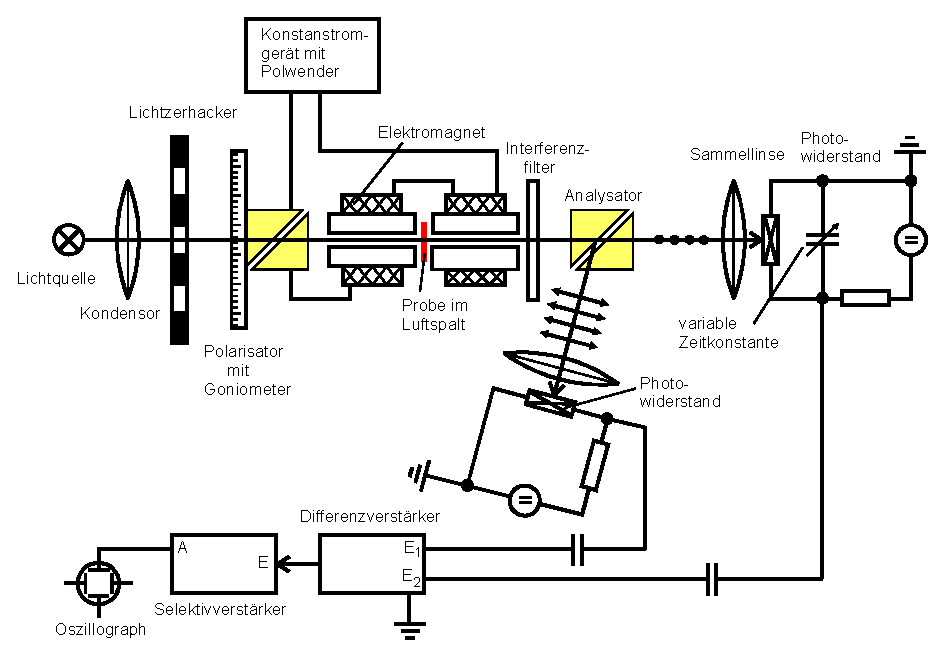
\includegraphics[width=0.8\textwidth]{Aufbau.pdf}
    \caption{Schematischer Versuchsaufbau \cite{ap46}.}
    \label{fig:aufbau}
\end{figure}

Bevor das Licht mittels eines Glan-Thompson-Prismas linear polarisiert wird, wird es von einem Lichtzerhacker gepulst. 
Dies dient dazu, das Hintergrundrauschen im späteren Verlauf durch einen Selektivverstärker zu eliminieren. Dafür wird der 
Selektivverstärker genau auf die Frequenz des Lichtzerhackers eingestellt. \\
\\
Hinter dem Prisma durchläuft das Licht den Magneten, in dessen Luftspalt sich die Probe befindet. Der Magnet wird von einem 
Konstantanstromgerät versorgt, sodass ein zeitlich konstantes Magnetfeld vorliegt. Das Magnetfeld lässt sich außerdem umpolen, um einen 
größeren Winkelbereich abzudecken. In der Probe dreht sich die Polarisationsebene des Lichts aufgrund des Faraday-Effekts. \\
\\
Hinter dem Magneten wird der Drehwinkel bei verschiedenen Wellenlängen untersucht. Dafür können neun 
verschiedene Interferenzfilter im Bereich von $1.06 \,\symup{\mu m}$ bis $2.65 \,\symup{\mu m}$ verwendet werden. Das Licht wird von einem weiteren 
Prisma in zwei linear polarisierte Wellen geteilt. Dessen Lichtintensität wird im Anschluss über jeweils einen Photowiderstand aus Bleisulfid gemessen. \\
\\
An einem Differenzverstärker werden die beiden Lichtintensitäten subtrahiert und verstärkt. An dem Selektivverstärker werden dann die Rauschspannungen 
herausgefiltert. Das gefilterte Signal wird nun auf einem Oszilloskop dargestellt.